%%
%% This is file `sample-sigconf.tex',
%% generated with the docstrip utility.
%%
%% The original source files were:
%%
%% samples.dtx  (with options: `sigconf')
%% 
%% IMPORTANT NOTICE:
%% 
%% For the copyright see the source file.
%% 
%% Any modified versions of this file must be renamed
%% with new filenames distinct from sample-sigconf.tex.
%% 
%% For distribution of the original source see the terms
%% for copying and modification in the file samples.dtx.
%% 
%% This generated file may be distributed as long as the
%% original source files, as listed above, are part of the
%% same distribution. (The sources need not necessarily be
%% in the same archive or directory.)
%%
%%
%% Commands for TeXCount
%TC:macro \cite [option:text,text]
%TC:macro \citep [option:text,text]
%TC:macro \citet [option:text,text]
%TC:envir table 0 1
%TC:envir table* 0 1
%TC:envir tabular [ignore] word
%TC:envir displaymath 0 word
%TC:envir math 0 word
%TC:envir comment 0 0
%%
%%
%% The first command in your LaTeX source must be the \documentclass
%% command.
%%
%% For submission and review of your manuscript please change the
%% command to \documentclass[manuscript, screen, review]{acmart}.
%%
%% When submitting camera ready or to TAPS, please change the command
%% to \documentclass[sigconf]{acmart} or whichever template is required
%% for your publication.
%%
%%
\documentclass[sigconf]{acmart}

%%
%% \BibTeX command to typeset BibTeX logo in the docs
\AtBeginDocument{%
  \providecommand\BibTeX{{%
    Bib\TeX}}}

%% Rights management information.  This information is sent to you
%% when you complete the rights form.  These commands have SAMPLE
%% values in them; it is your responsibility as an author to replace
%% the commands and values with those provided to you when you
%% complete the rights form.
\setcopyright{acmcopyright}
\copyrightyear{2024}
\acmYear{2024}
\acmDOI{XXXXXXX.XXXXXXX}

%% These commands are for a PROCEEDINGS abstract or paper.
\acmConference[ICoMS 2024]{7th International Conference on Mathematics and Statistics, ICoMS 2024}{June 23--25,
  2024}{Amarante, PT}
%%
%%  Uncomment \acmBooktitle if the title of the proceedings is different
%%  from ``Proceedings of ...''!
%%
%%\acmBooktitle{Woodstock '18: ACM Symposium on Neural Gaze Detection,
%%  June 03--05, 2018, Woodstock, NY}
\acmPrice{15.00}
\acmISBN{978-1-4503-XXXX-X/18/06}


%%
%% Submission ID.
%% Use this when submitting an article to a sponsored event. You'll
%% receive a unique submission ID from the organizers
%% of the event, and this ID should be used as the parameter to this command.
%%\acmSubmissionID{123-A56-BU3}

%%
%% For managing citations, it is recommended to use bibliography
%% files in BibTeX format.
%%
%% You can then either use BibTeX with the ACM-Reference-Format style,
%% or BibLaTeX with the acmnumeric or acmauthoryear sytles, that include
%% support for advanced citation of software artefact from the
%% biblatex-software package, also separately available on CTAN.
%%
%% Look at the sample-*-biblatex.tex files for templates showcasing
%% the biblatex styles.
%%

%%
%% The majority of ACM publications use numbered citations and
%% references.  The command \citestyle{authoryear} switches to the
%% "author year" style.
%%
%% If you are preparing content for an event
%% sponsored by ACM SIGGRAPH, you must use the "author year" style of
%% citations and references.
%% Uncommenting
%% the next command will enable that style.
%%\citestyle{acmauthoryear}


%%
%% end of the preamble, start of the body of the document source.
\begin{document}

%%
%% The "title" command has an optional parameter,
%% allowing the author to define a "short title" to be used in page headers.
\title{Longitudinal Feature Extraction in International Logistics Performance Index}

%%
%% The "author" command and its associated commands are used to define
%% the authors and their affiliations.
%% Of note is the shared affiliation of the first two authors, and the
%% "authornote" and "authornotemark" commands
%% used to denote shared contribution to the research.
\author{Aldina Correia}
\authornote{Both authors contributed equally to this research.}
\email{aic@estg.ipp.pt}
\orcid{0000-0002-4693-4867}
\authornotemark[1]
\affiliation{%
  \institution{CIICESI, ESTG, Instituto Politécnico do Porto}
  \streetaddress{Rua do Curral, Casa do Curral, Margaride}
  \postcode{4610-156}
  \city{Felgueiras}
  \country{Portugal}
}

\author{Diogo Ribeiro}
\email{diogo.ribeiro@mysense.ai}
\orcid{0009-0001-2022-7072}
\affiliation{%
  \institution{MySense}
  \streetaddress{7 Bell Yard}
  \postcode{WC2A 2JR}
  \city{London}
  \country{United Kingdom}}



%%
%% By default, the full list of authors will be used in the page
%% headers. Often, this list is too long, and will overlap
%% other information printed in the page headers. This command allows
%% the author to define a more concise list
%% of authors' names for this purpose.
\renewcommand{\shortauthors}{A. Correia and D. Ribeiro}

%%
%% The abstract is a short summary of the work to be presented in the
%% article.
\begin{abstract}
  The importance of the logistics performance of companies, regions and countries to support decision-making is universally recognised, covering the rationalisation of supply chains, the optimisation of inventory management and promoting global collaboration. 
      
  Efficient logistics integration with innovative technologies is crucial for the prompt delivery of materials and components, increasing the speed and effectiveness of innovation processes and, consequently, the performance of organisations. This study examines the robust correlation structure between Logistics Performance Index (LPI) indicators over several years. 
  
  The LPI assesses global logistical performance by measuring factors such as the quality of commercial and transport infrastructure, the ease of customs procedures and the efficiency of customs clearance, among other aspects that influence the transnational flow of goods.

Our results confirm the LPI as a longitudinal latent variable, characterised by its indicators, which demonstrate remarkable internal consistency. This consistency underpins the reliability of the LPI for assessing global logistics performance.

Recognised as a valuable measure of logistics efficiency, LPI serves as a practical tool in business and politics, guiding strategic decision-making and improving the operational cost-benefit ratio and competitiveness of organisations.
\end{abstract}

%%
%% The code below is generated by the tool at http://dl.acm.org/ccs.cfm.
%% Please copy and paste the code instead of the example below.
%%
\begin{CCSXML}
<ccs2012>
 <concept>
  <concept_id>10010520.10010553.10010562</concept_id>
  <concept_desc>Computer systems organization~Embedded systems</concept_desc>
  <concept_significance>500</concept_significance>
 </concept>
 <concept>
  <concept_id>10010520.10010575.10010755</concept_id>
  <concept_desc>Computer systems organization~Redundancy</concept_desc>
  <concept_significance>300</concept_significance>
 </concept>
 <concept>
  <concept_id>10010520.10010553.10010554</concept_id>
  <concept_desc>Computer systems organization~Robotics</concept_desc>
  <concept_significance>100</concept_significance>
 </concept>
 <concept>
  <concept_id>10003033.10003083.10003095</concept_id>
  <concept_desc>Networks~Network reliability</concept_desc>
  <concept_significance>100</concept_significance>
 </concept>
</ccs2012>
\end{CCSXML}

\ccsdesc[500]{Mathematics of computing~Probability and statistics~Probability and statistics~Statistical paradigms~Dimensionality reduction}
\ccsdesc[300]{Mathematics of computing~Probability and statistics~Probability and statistics~Multivariate statistics}
\ccsdesc[100]{Computing methodologies~Machine learning~Dimensionality reduction and manifold learning}

%%
%% Keywords. The author(s) should pick words that accurately describe
%% the work being presented. Separate the keywords with commas.
\keywords{Logistics Performance, LPI, Logistics Decision-Making, Feature Aggregation, Longitudinal Principal Component Analysis}
%% A "teaser" image appears between the author and affiliation
%% information and the body of the document, and typically spans the
%% page.

\received{20 February 2007}
\received[revised]{12 March 2009}
\received[accepted]{5 June 2009}

%%
%% This command processes the author and affiliation and title
%% information and builds the first part of the formatted document.
\maketitle

\section{Introduction}
Global logistics efficiency is crucial for companies considering international expansion. To assist with this, the World Bank has developed the Logistics Performance Index (LPI), which evaluates countries based on the quality of their trade infrastructure, ease of customs procedures, and efficiency of goods clearance across borders. The LPI is derived from surveys conducted with global freight forwarders and logistics professionals, capturing various facets of a country’s logistics environment[18].

The LPI measures logistics performance through six key dimensions:

\begin{itemize}
  \item \textbf{Customs Clearance Process:} Evaluates the efficiency of customs and border clearance \cite{arvis2016}.
  \item \textbf{Infrastructure Quality:} Assesses the quality of trade and transport infrastructure like ports and roads \cite{arvis2018}.
  \item \textbf{Ease of Arranging Shipments:} Looks at the ease of organizing competitively priced shipments \cite{arvis2016}.
  \item \textbf{Competence and Quality of Logistics Services:} Rates the skill and quality of logistics providers \cite{arvis2018}.
  \item \textbf{Tracking and Tracing:} Measures the ability to track and trace consignments \cite{arvis2016}.
  \item \textbf{Timeliness of Shipments:} Checks the regularity with which shipments meet delivery schedules \cite{arvis2018}.
\end{itemize}

Scores range from 1 to 5, with higher scores indicating superior logistics capabilities. This makes the LPI an invaluable tool for governments, businesses, and researchers to compare logistics performance internationally, spot improvement opportunities, and inform policy decisions \cite{worldbank2024}.

The 2023 LPI edition introduced new Key Performance Indicators (KPIs) based on big data, including real-time tracking of shipping containers, air cargo, and parcels, providing a broader perspective on global trade dynamics \cite{arvis2023}. These new KPIs complement traditional survey data, offering a fuller picture of logistics performance \cite{arvis2023}.

Proposals to enhance the LPI suggest various strategic improvements to better measure and optimize logistics conditions, especially important in scenarios where data collection might be compromised, such as during global disruptions \cite{rezaei2018, beysenbaev2020}.

The LPI thus not only aids businesses in making informed decisions about international operations but also helps countries in developing policies that foster an efficient logistics framework. The 2023 edition of the International Logistics Performance Index (LPI) enables comparisons across 139 countries, revealing an overall improvement in global logistics performance over the past decade \cite{arvis2023}. Notably, the LPI score increased, with a secondary peak emerging around 3.5 between 2018 and 2023, indicating stronger performance among more countries. However, the reduction in sample size from 160 countries in 2018 to 139 in 2023 complicates direct comparisons, especially at the lower score ranges \cite{arvis2023}.

The LPI consistently evaluates a broad spectrum of economies, though the specific countries assessed can vary in each edition due to data availability and varying participation levels. For instance, the 2014 edition did not include data for Portugal.

In 2023, the highest LPI scores were predominantly from high-income economies, with Singapore maintaining its top ranking from previous years with a score of 4.3. Eight of the top twelve scorers were European countries. Conversely, the lowest scores generally came from countries with low to lower-middle incomes facing economic challenges from conflicts, natural disasters, or geographic and economic constraints, affecting their integration into global supply chains.

This paper aims to validate the LPI as a reliable measure of logistical performance by analyzing key characteristics and relationships among its indicators. Recognizing the LPI as a robust metric allows it to inform strategic decision-making in engineering and other sectors, improving operational cost-effectiveness and competitiveness. Additionally, the paper tracks Portugal’s LPI performance from 2007 to 2023, focusing on its changes and implications for logistics strategy.

\section{Introduction 2}
Global logistics efficiency is increasingly crucial for companies considering international expansion. As globalization deepens, the ability of businesses to efficiently move goods across international borders becomes pivotal to maintaining competitive advantage. The World Bank recognizes this and has developed the Logistics Performance Index (LPI), an interactive benchmarking tool designed to help countries identify challenges and opportunities in their trade logistics performance and improve upon them \cite{WBreport2018}.

The LPI is an aggregate indicator that assesses diverse factors affecting the logistics environment in countries globally. Derived from surveys conducted with worldwide logistics professionals, the LPI encapsulates expert evaluations of international freight forwarding and express carriers. It serves to highlight the performance of countries in six key dimensions: customs performance, infrastructure quality, ease of arranging shipments, logistics services quality, consignments tracking and tracing, and timeliness of shipments \cite{WBreport2018}. These dimensions combine the weighted average of country scores with practical data measuring logistics efficiency, indicating the relative ease and efficiency with which products can be moved into and inside a country \cite{WBreport2018}.

Singapore and Finland were ranked as the most efficient and highest LPI countries in the 2023 edition of the index \cite{worldbank4}. Historically, the LPI was reported by the World Bank every two years from 2010 to 2018, with a hiatus in 2020 due to the COVID-19 pandemic and a restructuring of the index methodology, eventually releasing again only in 2023. The survey-based approach has been complemented since 2023 with certain Key Performance Indicators (KPIs) and Big Data to enhance the results \cite{WBreport2018}.

Scores on the LPI range from 1 to 5, with higher scores indicating more effective logistics systems. These scores are invaluable for businesses planning global expansion strategies as they highlight potential logistical barriers and opportunities in target markets. The 2023 edition of the LPI, for instance, introduced new KPIs based on big data sources including real-time tracking of shipping containers, air cargo, and parcels. This integration of big data brings a broader perspective on global trade dynamics, making the LPI an even more robust tool for strategic decision-making \cite{arvis2023}.

Moreover, the LPI assists policymakers and researchers by providing a benchmarking tool to compare logistics performance internationally. Such comparisons are critical for identifying improvement opportunities and informing policy decisions aimed at enhancing trade logistics, thereby fostering economic growth. Proposals to enhance the LPI suggest various strategic improvements to better measure and optimize logistics conditions, especially important in scenarios where data collection might be compromised, such as during global disruptions \cite{rezaei2018, beysenbaev2020}.

The latest insights from the 2023 LPI indicate an overall improvement in logistics performance globally, although variations remain significant among different regions and income levels. High-income countries typically score well, reflecting robust infrastructure and efficient customs procedures, while lower-income nations often lag, hindered by various challenges ranging from infrastructural deficiencies to bureaucratic complexities \cite{arvis2023}.

LPI results have been used in many policy reports and documents prepared by multilateral organizations and findings from the index provide a worldwide general benchmark for the logistics industry and for logistics users \cite{WBreport2018}. These results have also been embraced by the academic community, highlighting the LPI's importance beyond just the professional logistics sphere.

This paper seeks to validate the LPI as a reliable measure of logistical performance by analyzing key characteristics and relationships among its indicators. By recognizing the LPI as a comprehensive and robust metric, it can be employed to inform strategic decision-making across engineering, logistics, and policy sectors, thereby enhancing operational efficiency and competitiveness on a global scale.

\section{Introduction 3}
Thanks to to the globalisation of production, the speed and efficiency with which company’s can move goods across international boarders has become a key feature of their global competitiveness. This is reflected by the continuing importance of measures such as the World Bank’s Logistics Performance Index (LPI).

The LPI, an index compiled by the World Bank, ‘measures the performance of countries’ logistics system (ease of arranging competitively priced shipments) and provides a guide for businesses and policymakers interested in global trade’ and international investments. The LPI allows countries to ‘assess their current logistics-related strengths and weaknesses, identify the areas in which they need to improve, and benchmark their performance against global standards to enhance their international trade capabilities \cite{WBreport2018}.


The LPI is an aggregate indicator that assesses diverse factors affecting the logistics environment in countries globally. Derived from surveys conducted with worldwide logistics professionals, the LPI encapsulates expert evaluations of international freight forwarding and express carriers. It serves to highlight the performance of countries in six key dimensions: customs performance, infrastructure quality, ease of arranging shipments, logistics services quality, consignments tracking and tracing, and timeliness of shipments \cite{WBreport2018}. These dimensions combine the weighted average of country scores with practical data measuring logistics efficiency, indicating the relative ease and efficiency with which products can be moved into and inside a country \cite{WBreport2018}.

The importance of the LPI stems from its reflection of the quality and efficiency of a nation's logistics system, which impacts trade performance, economic growth, and social development. A high LPI score facilitates faster, cheaper, and more reliable movement of goods, enhancing competitiveness and market access. Conversely, a low LPI score implies higher costs, delays, and risks, reducing a country's trade potential and attractiveness. The LPI also serves as a critical tool for monitoring progress and the impacts of reforms and investments in logistics.

Improving the LPI requires a comprehensive and coordinated approach that addresses various factors impacting a logistics system. Simplifying and harmonizing customs procedures and regulations can significantly reduce the time and cost associated with clearing goods at the border. Investments in transport infrastructure, diversification of international shipment options, and optimization of shipment modes enhance connectivity, reliability, flexibility, and affordability of logistics networks. Further investments in human resources, technology, and innovation can bolster the quality and competence of logistics services. The adoption of digital platforms and tools for better tracking and tracing improves the visibility and security of cargo movements. Moreover, reducing variability and uncertainty in logistics operations enhances timeliness in delivery \cite{WBreport2018}.

Monitoring the LPI is essential for evaluating performance, identifying gaps, and tracking progress. This involves comparing LPI scores and rankings with other countries, analyzing strengths and weaknesses by dimension, reviewing changes over time to assess the impact of logistics reforms, and soliciting feedback from stakeholders to validate and complement LPI data \cite{WBreport2018}.

Learning from the LPI enables countries to leverage opportunities, address challenges, and enhance competitiveness and resilience. Accessing detailed analyses and recommendations from LPI reports, joining the LPI community of practice, and participating in events and webinars are vital steps for engaging with global best practices and the latest innovations in logistics \cite{worldbank4}.

Singapore and Finland were ranked as the most efficient and highest LPI countries in the 2023 edition of the index \cite{worldbank4}. The LPI assists policymakers and researchers by providing a benchmarking tool to compare logistics performance internationally. These comparisons are critical for identifying improvement opportunities and informing policy decisions aimed at enhancing trade logistics, thereby fostering economic growth \cite{arvis2023}.

The latest insights from the 2023 LPI indicate an overall improvement in logistics performance globally, although variations remain significant among different regions and income levels \cite{arvis2023}. High-income countries typically score well, reflecting robust infrastructure and efficient customs procedures, while lower-income nations often lag, hindered by various challenges ranging from infrastructural deficiencies to bureaucratic complexities.

This paper seeks to validate the LPI as a reliable measure of logistical performance by analyzing key characteristics and relationships among its indicators. By recognizing the LPI as a comprehensive and robust metric, it can be employed to inform strategic decision-making across engineering, logistics, and policy sectors, thereby enhancing operational efficiency and competitiveness on a global scale.

\section{Introduction 4}
Thanks to to the globalisation of production, the speed and efficiency with which company’s can move goods across international boarders has become a key feature of their global competitiveness. This is reflected by the continuing importance of measures such as the World Bank’s Logistics Performance Index (LPI).

The LPI, an index compiled by the World Bank, ‘measures the performance of countries’ logistics system (ease of arranging competitively priced shipments) and provides a guide for businesses and policymakers interested in global trade’ and international investments. The LPI allows countries to ‘assess their current logistics-related strengths and weaknesses, identify the areas in which they need to improve, and benchmark their performance against global standards to enhance their international trade capabilities.


The LPI is an aggregate index for a welfare evaluation of countries’ logistics performance worldwide based on multiple variables. The LPI is derived from a survey of international freight forwarders and express carriers around the world and is an overall impression of countries’ performance in six key areas: (1) customs performance; (2) infrastructure quality; (3) logistics service quality; (4) ease of arranging competitively priced shipments; (5) consignment tracking and tracing; and (6) timeliness (speed). The scores for each of these aspects of logistics performance are weighted averages of country scores and hard data that capture logistic efficiency by quantifying the ease with which goods cross borders and circulate in the country, that is, to allow goods to flow into, and to transit within, the country in a speedy and cost-efficient manner.


\section{Data and Results}

The LPI \cite{WB} index is calculated from 6 indicators or six key dimensions \cite{WBreport2016,WBreport2018}:
\begin{enumerate}
    \item \textbf{Customs} Clearance Process: The efficiency of customs and border clearance processes.
    \item \textbf{Infrastructure} Quality: The quality of trade and transport-related infrastructure, including ports, railroads, and roads.
    \item Ease of Arranging \textbf{(International) Shipments}: The ease of arranging competitively priced shipments.
    \item \textbf{Logistics Competence and Quality } of Services: The competence and quality of logistics services, such as transport operators and customs brokers.
    \item \textbf{Timeliness} of Shipments: The frequency with which shipments reach the consignee within the scheduled or expected delivery time.
    \item \textbf{Tracking and Tracing}: The ability to track and trace consignments.
\end{enumerate}

To identify the variables that most contribute  to the countries' logistical performance, techniques for selecting or extracting key indicators can be used. In both cases, the aim is to retain the indicators that maximise the variance extracted from the original data.

In \cite{correiaICIE}, to ensure that the extracted characteristics were relevant and informative in relation to the 2023 Logistics Performance Index indicators, extraction techniques were used, in particular Exploratory Factor Analysis (EFA) in the JASP \cite{JASP} software.

The present study considers LPI indicators over several years, being therefore a longitudinal approach, using the software R \cite{R}.

This analysis is based on the values of the LPI \cite{BM} indicators in the years 2007, 2010, 2012, 2014, 2016, 2018 and 2023.

As the EFA carried out in \cite{correiaICIE} allowed the identification of a single factor, in this work a Principal Component Analysis (PCA) was carried out over the available years, considering one component.

Assumptions for this techniques (EFA and PCA)  are: (i) sample dimension -- 5 to 10 observations by variable; (ii) normality of the variables; (iii) linearity of the variables; (iv) homocedasticity.

(i) Sample dimension - The sample comprises between 139 and 160 countries (Table \ref{tab:kmo}), and there is no missing values. Therefore, the sample size is adequate for the analysis of the six indicators.

\begin{table*}[h]
  \caption{Kaiser-Meyer-Olkin and MSA}
  \label{tab:kmo}
\begin{tabular}{lccccccc}
\toprule
\textbf{Indicator (Score)}	&	\textbf{2007}	&	\textbf{2010}	&	\textbf{2012}	&	\textbf{2014}	&	\textbf{2016}	&	\textbf{2018}	&	\textbf{2023}	\\  
\midrule
Customs	&	0.91	&	0.92	&	0.93	&	0.89	&	0.95	&	0.95	&	0.91	\\	
Infrastructure	&	0.90	&	0.88	&	0.94	&	0.91	&	0.93	&	0.92	&	0.90	\\	 
International Shipments	&	0.96	&	0.98	&	0.96	&	0.97	&	0.96	&	0.96	&	0.97	\\	 
Logistics Competence and Quality	&	0.93	&	0.89	&	0.91	&	0.91	&	0.93	&	0.91	&	0.93	\\	 
Timeliness	&	0.97	&	0.98	&	0.96	&	0.94	&	0.94	&	0.96	&	0.94	\\	 
Tracking and Tracing	&	0.93	&	0.94	&	0.94	&	0.93	&	0.94	&	0.95	&	0.92	\\	 
\midrule
KMO - Overall MSA	&	0.93	&	0.92	&	0.94	&	0.92	&	0.94	&	0.94	&	0.93	\\	 
\midrule
Number of Countries	&	150	&	155	&	155	&	160	&	160	&	160	&	139\\	
\bottomrule
\end{tabular}
\end{table*}

(ii) Normality Assessment - Both the Mardia Test and the Energy Test were used, under the null hypothesis of multivariate normality.
In some year Mardia's Test presented p values greater than 0.05, therefore, a multivariate normal distribution can be considered, but in most years none of the tests allows to confirm this assumption.

(iii) Linearity -- Pearson's Correlations between Indicators are significant at the 5\% significance level, in addition, they are all high, exceeding the value of 0.8, suggesting a strong interdependence between them (multicollinearity).
Consequently, the extraction of factors from these characteristics is justified and imperative, in order to exclude potential redundancies and increase the robustness of the analysis.

(iv) Homoscedasticity -- The standard deviation values of the indicators are close to and below 1, which suggests the existence of homoscedasticity and a relatively consistent distribution of data around the respective means for each indicator, over the years.

Once the necessary conditions have been verified, PCA can be implemented to extract the principal component that maximises the retention of variance of the observed variables.

%----- Requires booktabs package -----%
The Kaiser-Meyer-Olkin (KMO) Measure of Sample Adequacy (MSA) or Overal MSA and the MSA for each variable indicates the suitability of the variable for PCA. 

KMO ranges between 0.92 and 0.94, over the years
and the individual MSA of each variable between 0.88 and 0.98.
This all individual MSAs are greater than the 0.5 threshold, indicating that they are adequate for the analysis. Additionally, the overall MSA or KMO  values suggests excellent suitability for applying PCA \cite{maroco2018analise}. 


\textcolor{red}{FALTAM OS RESULTADos}
The chi-square goodness-of-fit test, with null hypothesis that the observed data correlation matrix  is a random sample realisation from population having correlation matrix equal to the one returned by the extracted factors, has the $\chi^2$ presented in Table \ref{tab:loadings}, with $df=9$ and a $p-value <0.001$.


In determining the number of factors to retain by focusing on PCA eigenvalues  exceeding 1 (\cite{carroll1978effect}), a single factor was extracted  over the years. The percentage of variance retained of these indicators over the years is between 87.8 and 94.4 (Table \ref{tab:loadings}). Within this factor,  Logistics Competence and Quality is always the indicator with highest loading. The behaviour of the loading's values across the time can be observed in Table \ref{tab:loadings} and Figure \ref{fig:PCAl}.

\begin{figure*}
    \centering
    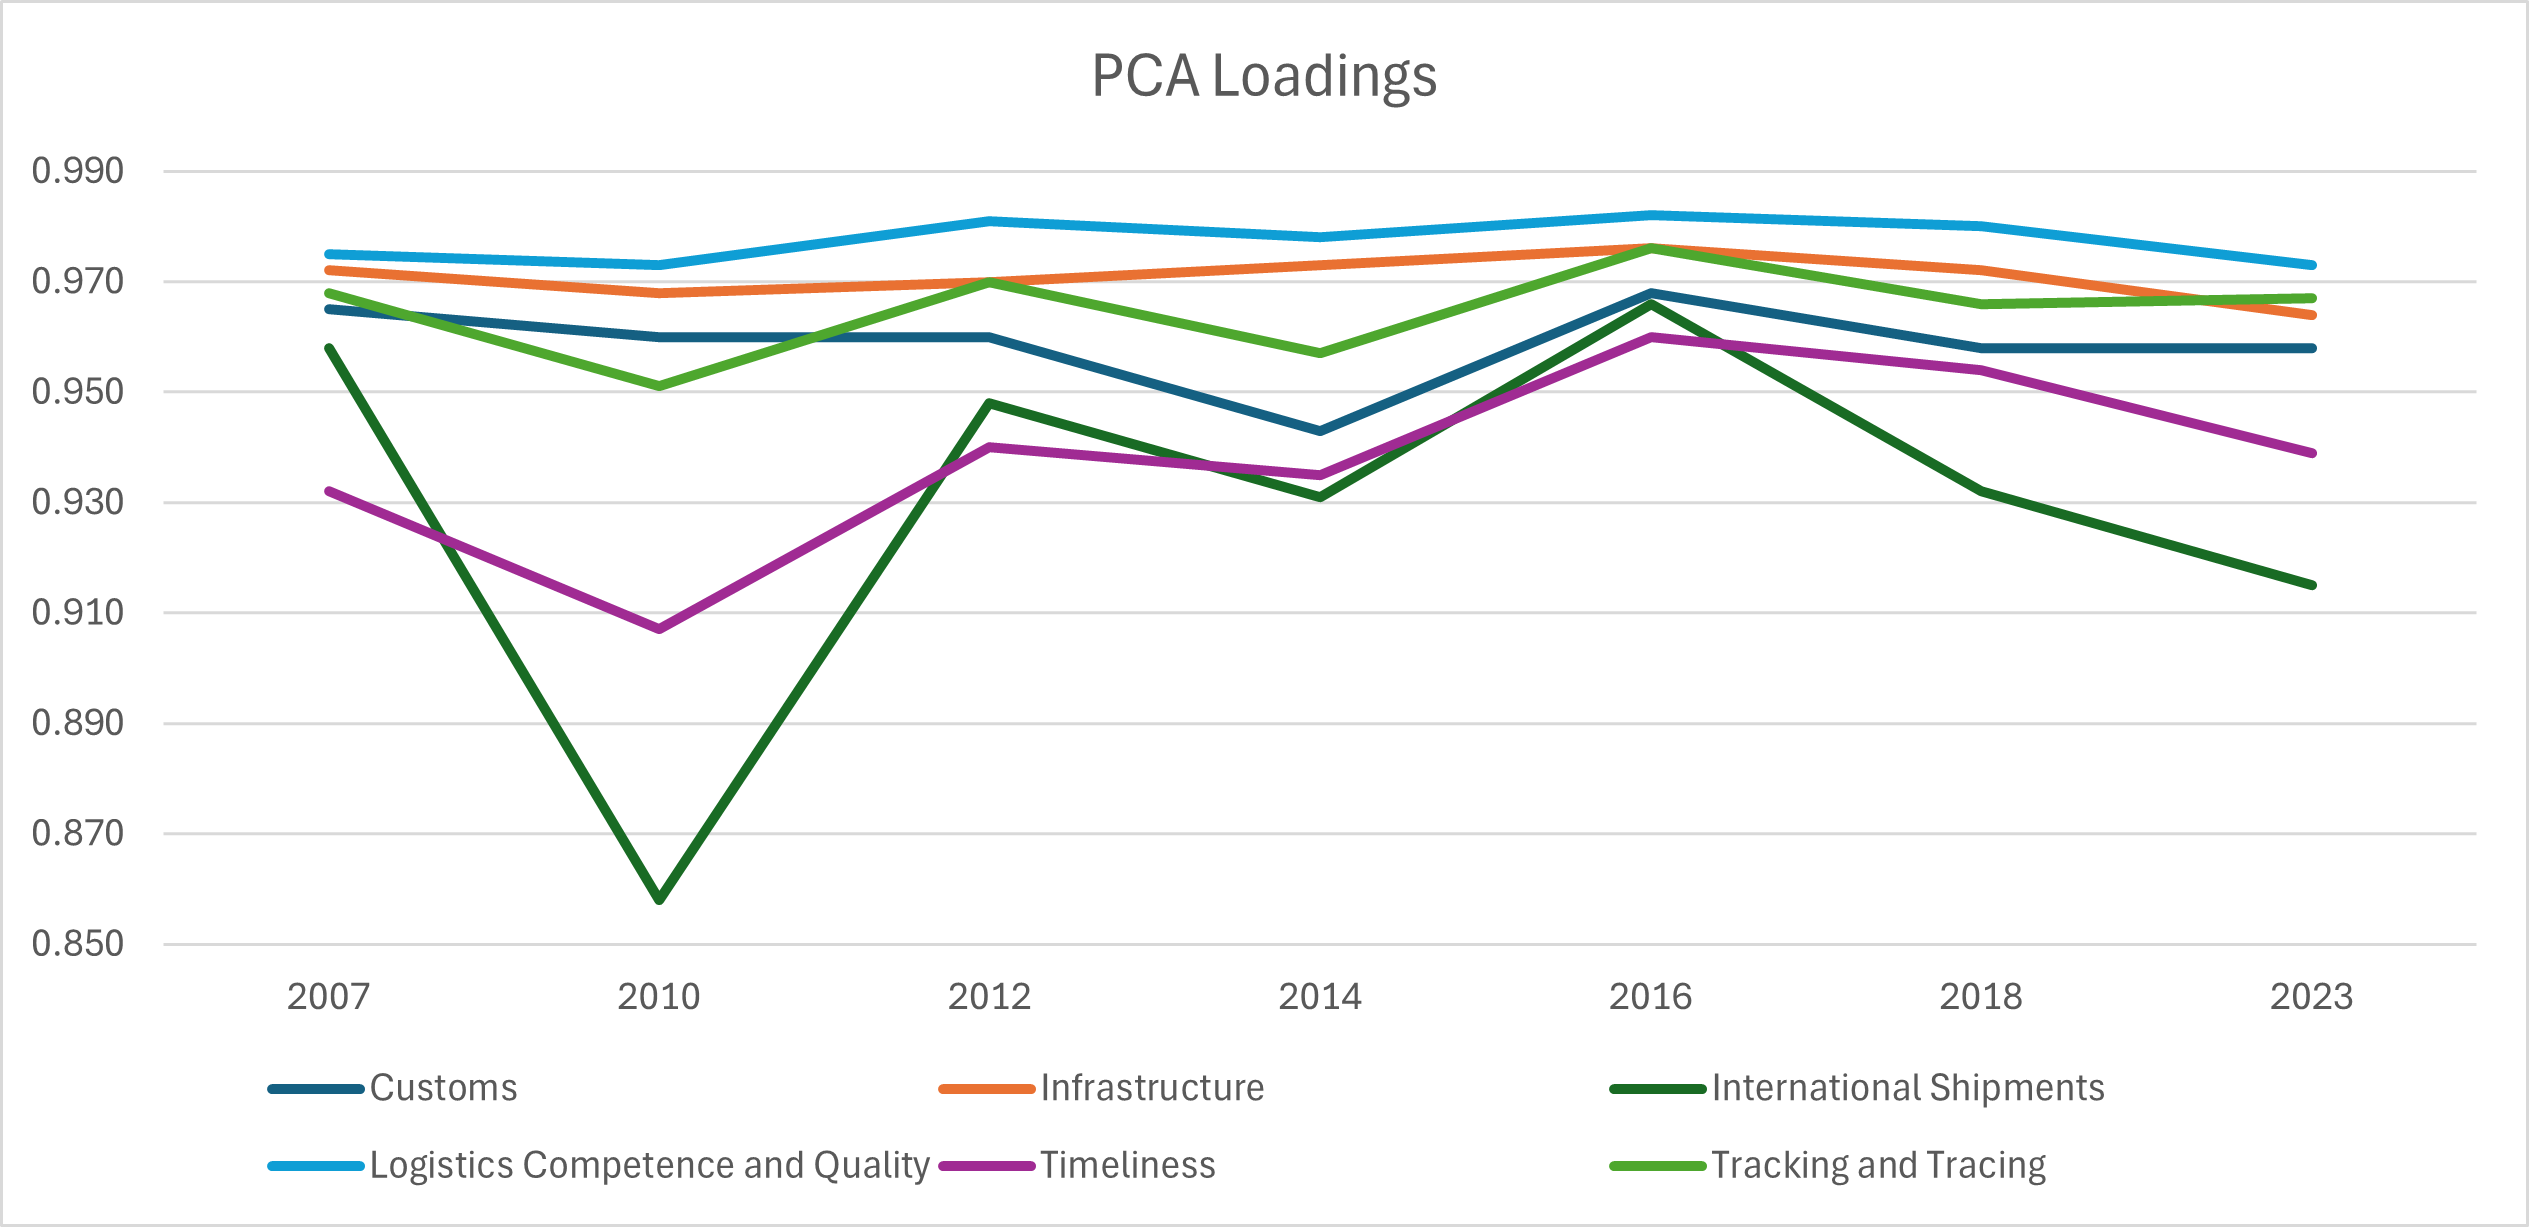
\includegraphics[width=0.7\textwidth]{Loadings.png}
    \caption{PCA Loadings across the years}
    \label{fig:PCAl}
\end{figure*}

\textcolor{red}{AQUI-------------------}
The reliability of factors in the context of factor analysis refers to the consistency or stability of the measurement of underlying constructs represented by those factors. There are several ways to assess the reliability of factors, being the commonly used measure the Cronbach's Alpha, a frequentist scale Reliability Statistics. It assesses how well the items within a factor consistently measure the same underlying construct. A higher Cronbach's alpha value (typically above 0.70) indicates greater reliability.
%


\begin{table*}[h]
  \caption{PCA Loadings, Explaned Variance and Reliability}
  \label{tab:loadings}
\begin{tabular}{lccccccc}
\toprule
\textbf{Indicator (Score)}	&	\textbf{2007}	&	\textbf{2010}	&	\textbf{2012}	&	\textbf{2014}	&	\textbf{2016}	&	\textbf{2018}	&	\textbf{2023}	\\  
\midrule
Customs	&	0.965	&	0.960	&	0.960	&	0.943	&	0.968	&	0.958	&	0.958	\\	
Infrastructure	&	0.972	&	0.968	&	0.970	&	0.973	&	0.976	&	0.972	&	0.964	\\	
International Shipments	&	0.958	&	0.858	&	0.948	&	0.931	&	0.966	&	0.932	&	0.915	\\	
Logistics Competence and Quality	&	0.975	&	0.973	&	0.981	&	0.978	&	0.982	&	0.980	&	0.973	\\	
Timeliness	&	0.932	&	0.907	&	0.940	&	0.935	&	0.960	&	0.954	&	0.939	\\	
Tracking and Tracing	&	0.968	&	0.951	&	0.970	&	0.957	&	0.976	&	0.966	&	0.967	\\	\midrule
Explaned Variance (\%) - 1 factor 	&	92.5	&	87.8	&	90.8	&	92.4	&	94.3	&	92.3	&	90.8	\\	\midrule
Reliability - Cronbach' $\alpha$	&	0.983	&	0.970	&	0.982	&	0.979	&	0.987	&	0.982	&	0.978	\\	\bottomrule
\end{tabular}
\end{table*}

The estimate Cronbach's $\alpha$ of the factor obtained in this EFA is $0.978$, indicating excelent reliability (\cite{pestana2008analise}). Additionally, even if an item is dropped, the frequentist individual item of reliability (see Table \ref{tab:reliability}) remain very high. This suggests that each individual item significantly contributes to the overall reliability of the factor, confirming the exceptional internal consistency of the measures employed. This internal consistency is crucial to ensure the reliability and validity of the analysis results. 
Consequently, this provides evidence of the excellent internal consistency of the latent variable.


\section{Conclusion and Future Work}

In this study, a comprehensive examination revealed a strong correlation among all the indicators encompassed within the Logistics Performance Index (LPI). This observation suggests that the LPI can be conceptualized as a latent variable, representing an underlying construct with remarkable internal consistency, as elucidated by its constituent indicators. The high level of correlation among these indicators implies a coherent and unified measurement of the latent variable, reinforcing the reliability and coherence of the LPI as a robust tool for assessing logistics performance. This insight contributes to a nuanced understanding of the interrelationships among the various dimensions captured by the LPI, providing a solid foundation for further analysis and interpretation of logistics performance on both a national and global scale.
Verifiing LPI as a reliable indicator of countries' logistical performance enables its utilization in engineering as a valuable source of practical insights for innovation. It guides optimal strategic decision-making, providing a comprehensive view of a nation's logistical capabilities, including infrastructure, process efficiency, and transportation services. By using LPI as a source of practical knowledge, governments, companies and engineers can identify specific opportunities and challenges related to logistics in various geographic contexts. For example, a country ranking high on the LPI may indicate an environment conducive to the development of new transportation technologies or efficient supply chains. Conversely, a low LPI score may flag areas where engineering interventions are needed to improve transportation infrastructure or optimize logistics processes.

Concerning with Portugal's performance over the period from 2007 to 2023, particularly, focusing on its overall LPI score, has remained consistent since 2007, although its global ranking has undergone fluctuations. In 2007, Portugal ranked within the top 18\%, improving to the top 14\% by 2018. However, in 2023, Portugal dropped to the 38th position, reflecting a dynamic shift. During that year, 27\% of the 139 assessed countries surpassed Portugal's LPI. 

As mentioned in the LPI reports, for example \cite{WBreport2016,WBreport2018}, but namely in the 2023 report \cite{WBreport2023}, several dimensions of the logistic performance can be out of this index, they try to include other KPI in the index, or to complete information with other type of indicators. It can be a good suggestion for future work. Also to develop a logistic performance index for logistic companies and extend these concepts to the industrial level would be very useful for these companies.


As highlighted in the LPI reports, such as those in 2016 and 2018 \cite{WBreport2016, WBreport2018}, and particularly in the 2023 report \cite{WBreport2023}, various dimensions of logistic performance may fall outside the scope of this index. Efforts have been made to incorporate additional Key Performance Indicators into the index or supplement information with other types of indicators. This observation provides valuable insights for potential future research. Furthermore, the suggestion to develop a logistic performance index tailored specifically for logistics companies and extend these concepts to the industrial level could be highly beneficial for such entities.




%%
%% The acknowledgments section is defined using the "acks" environment
%% (and NOT an unnumbered section). This ensures the proper
%% identification of the section in the article metadata, and the
%% consistent spelling of the heading.
\begin{acks}
This work has been supported by national funds through FCT - Fundação para a Ciência e Tecnologia through project UIDB/04728/2020.
\end{acks}

%%
%% The next two lines define the bibliography style to be used, and
%% the bibliography file.
\bibliographystyle{ACM-Reference-Format}
\bibliography{sample-base}


%%
%% If your work has an appendix, this is the place to put it.
\appendix

\section{appendix A}

\subsection{Part One}

Lorem ipsum dolor sit amet, consectetur adipiscing elit. Morbi
malesuada, quam in pulvinar varius, metus nunc fermentum urna, id
sollicitudin purus odio sit amet enim. Aliquam ullamcorper eu ipsum
vel mollis. Curabitur quis dictum nisl. Phasellus vel semper risus, et
lacinia dolor. Integer ultricies commodo sem nec semper.

\subsection{Part Two}

Etiam commodo feugiat nisl pulvinar pellentesque. Etiam auctor sodales
ligula, non varius nibh pulvinar semper. Suspendisse nec lectus non
ipsum convallis congue hendrerit vitae sapien. Donec at laoreet
eros. Vivamus non purus placerat, scelerisque diam eu, cursus
ante. Etiam aliquam tortor auctor efficitur mattis.

\section{Appendix B}

Nam id fermentum dui. Suspendisse sagittis tortor a nulla mollis, in
pulvinar ex pretium. Sed interdum orci quis metus euismod, et sagittis
enim maximus. Vestibulum gravida massa ut felis suscipit
congue. Quisque mattis elit a risus ultrices commodo venenatis eget
dui. Etiam sagittis eleifend elementum.

Nam interdum magna at lectus dignissim, ac dignissim lorem
rhoncus. Maecenas eu arcu ac neque placerat aliquam. Nunc pulvinar
massa et mattis lacinia.

\end{document}
\endinput
%%
%% End of file `sample-sigconf.tex'.
